\chapter{Design and Implementation}\label{ch:implementation}
Implementation goes here.\todo{write an intro here}

\section{Preliminary Interest Test}
For the purpose of testing different methods of data gathering for the evaluation a preliminary test was conducted. This test also served the purpose of obtaining a baseline for the length of time users might spend on an AR application, which also served as an answer to research question 1.

\subsection{Metrics}\label{subsec:premetrics}
For this test four different sets of data were gathered. Two of the metrics were self-reporting, meaning the participant chose the answer. The other two metrics were data gathered by the sensors attached to the arduino and to the participant. The four parameters are as follows:
\paragraph{Electrodermal activity (EDA):} The EDA sensors measure the skin conductance of the wearer. This is used to read the wearer’s level of arousal, which rise and fall depending on the task of the wearer and how exciting they find the task. The more aroused the wearer is, the more sweat will be generated and thereby increasing the conductance.
\paragraph{Inter-Beat interval (IBI):} The IBI sensor measures the heart rate variability (HRV) which varies from beat to beat, by recording the beats of the pulse. The more relaxed a person is the more variability there is between the beats, and vice versa. 
\paragraph{Time:} Throughout the experiment, the time is recorded so that other parameters may be compared to it. This was done by having the facilitator stop the timer when receiving a notice from the participant to stop, since the equipment work by the participant during the test prohibited them from stopping the timer themselves.
\paragraph{Self-assessment manikin (SAM):} As described by Bradley and Lang (1994), the \textit{self-assessment manikin} (SAM) is a picture-oriented instrument to assess a subject’s pleasure, arousal, and feeling of control in response to a stimulant. The three rows, seen in Figure \ref{fig:SAM}, each represent one of these parameters on a 5-point scale with graphic depictions \cite{Bradley1994}. Subjects may point at the image which best represents their feeling of pleasure, arousal, and control.

\begin{figure}[h!]
    \centering
    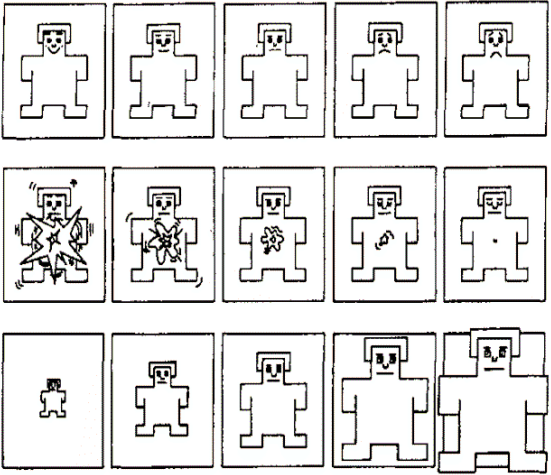
\includegraphics[width=\textwidth]{figures/SAM.png}
    \caption{The three SAM scales: Pleasure (top), arousal (middle), and control (bottom) \cite{Bradley1994}}\label{fig:SAM}
\end{figure}

\subsection{Setup}
The following tools are used for the purposes of the preliminary interest test:

\begin{itemize}
    \item A smartphone with the AR app \textit{AR Dino Roar} installed
    \item An arduino with breadboard (as well as the necessary wires to connect everything)
    \item Two EDA sensors
    \item A pulse sensor
    \item A smartphone to serve as a stopwatch
    \item A computer to which the arduino is connected
    \item A camera to film the procedure
    \item A piece of paper with a pattern to serve as an AR marker
    \item A piece of paper showing the SAM scales
\end{itemize}

\textit{AR Dino Roar} is an application for android devices in which users may use their own pattern as an AR marker. The app then displays a model of a dinosaur in AR. A screenshot of this app can be seen in Figure \ref{fig:dino}.

\begin{figure}[h!]
    \centering
    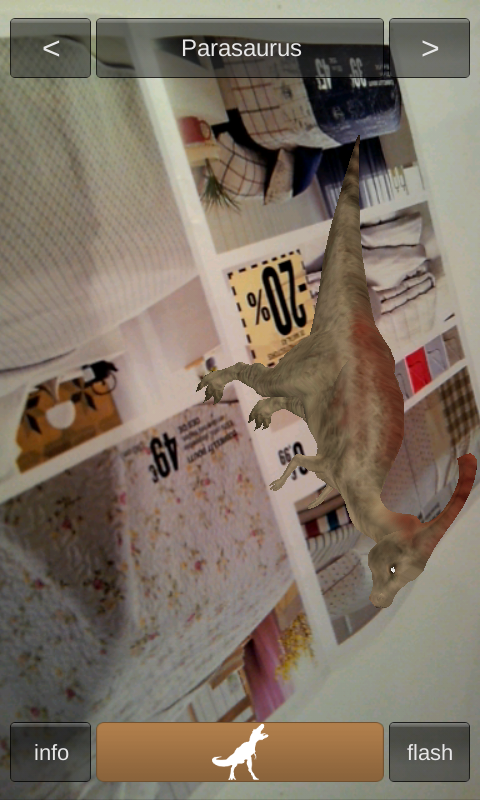
\includegraphics[scale=0.3]{figures/AR_dino.png}
    \caption{A screenshot of the AR Dino Roar app \cite{ARDino}}\label{fig:dino}
\end{figure}

In the test setup, a circuit is set up with the arduino, breadboard, sensors and wires in such a way that one can measure a participant’s EDA and IBI. The arduino is connected to the computer so that this data may be recorded. The EDA sensors are attached to the left index and middle finger of the participant, and the pulse sensor is attached to their left ear lobe, as seen in Figure \ref{fig:pretest_ear}.

\begin{figure}[h!]
    \centering
    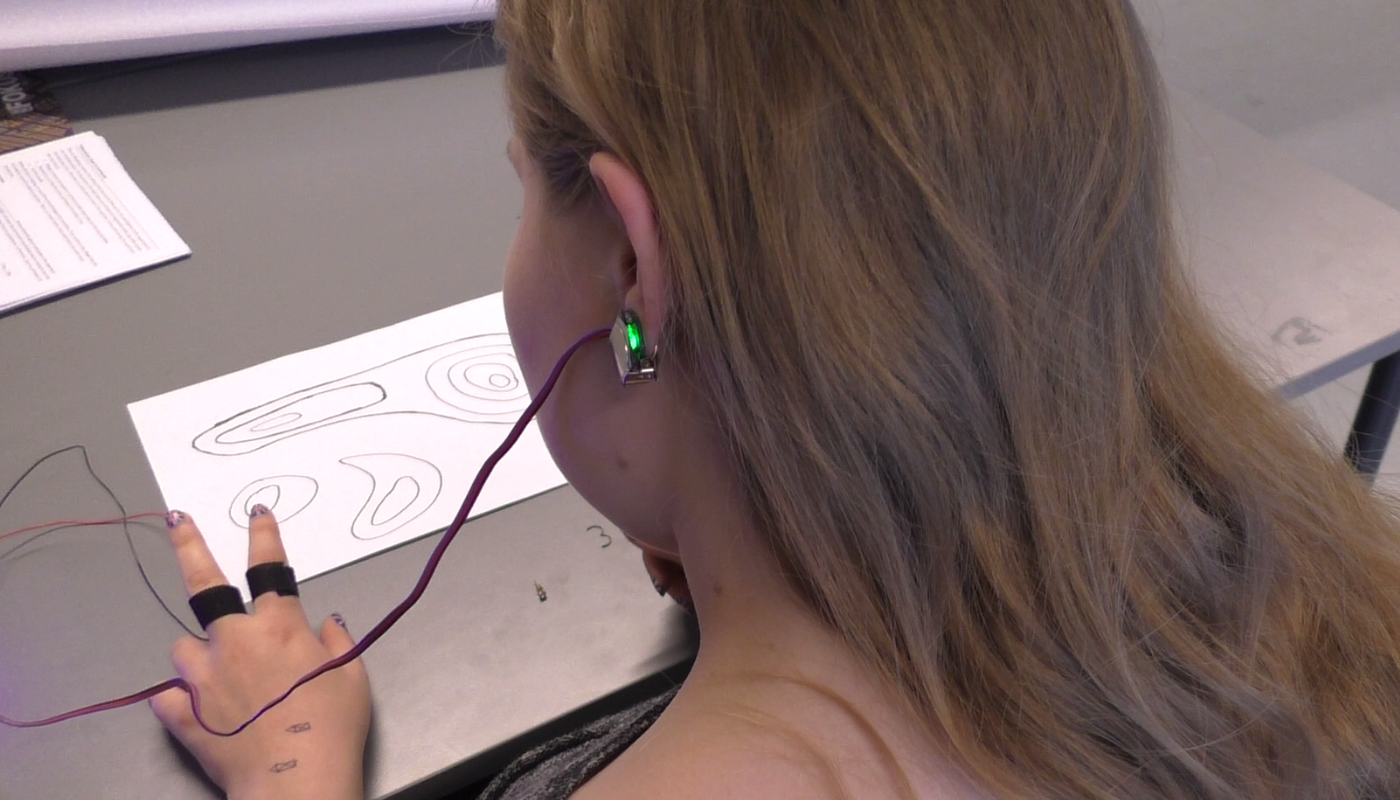
\includegraphics[width=0.6\textwidth]{figures/pretest_ear.png}
    \caption{The EDA and pulse sensors attached to a participant}\label{fig:pretest_ear}
\end{figure}

The test participant is seated in front of a table. On this table is the AR marker, the two smartphones, the SAM paper, and the arduino to which the participant is connected. The test facilitator is seated next to the participant in front of a computer, on which they record results from the test. The full test setup can be seen in Figure \ref{fig:pretest_setup}.

\begin{figure}[h!]
    \centering
    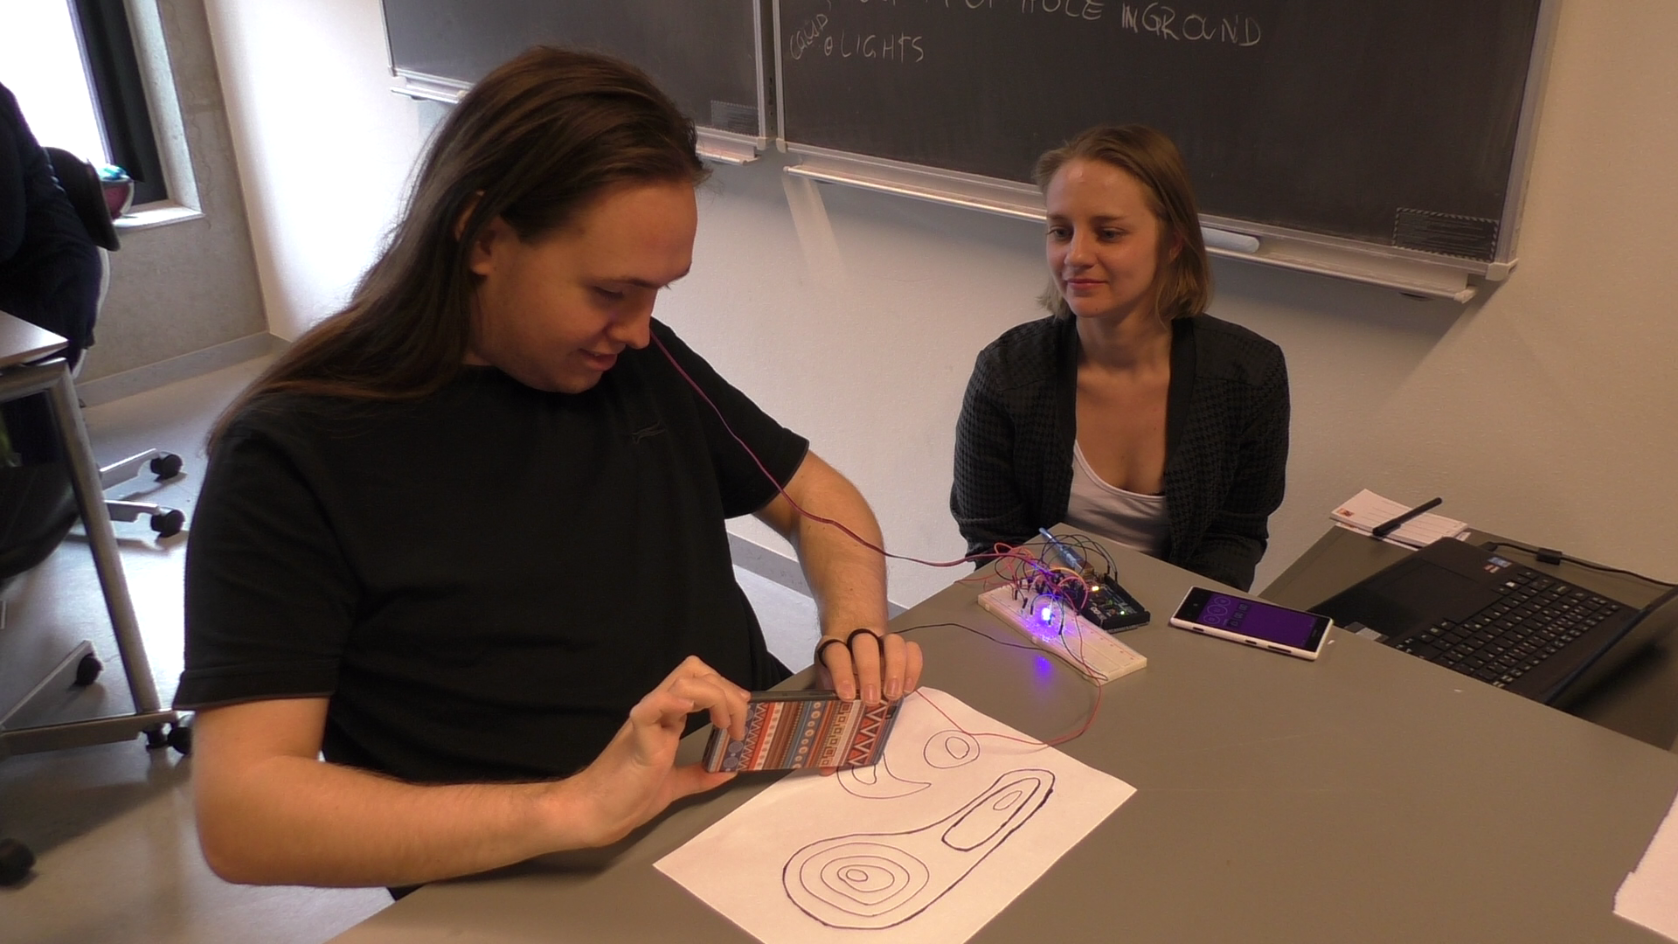
\includegraphics[width=0.6\textwidth]{figures/pretest_setup.png}
    \caption{The setup for the preliminary interest test}\label{fig:pretest_setup}
\end{figure}

\subsection{Procedure}
Before the test begins, the facilitator explains the procedure to the participant. They then attach the sensors to the participant as described in the previous section. Before the participant interacts with anything, they must sit idly for one minute, so that a baseline IBI and EDA may be recorded. They are then asked to use the AR Dino Roar app to look at a virtual dinosaur. The stopwatch is started once they begin, and they are asked to tell the facilitator to stop the timer once they are no longer interested in the app. Their IBI and EDA is recorded while they interact with the app. Once they are done interacting with the app, they are asked to answer three questions using the SAM diagram: how pleased, aroused, and in control they felt, respectively. For each question, they were asked to point to one of five images in a given row which best described their feelings, as described in section \ref{subsec:premetrics}.

\subsection{Analysis of results}
Out of the ten tests only seven sets of data were usable in regards to the logging of the sensor data. At some point after test number 5, something happened to make the data unstable and faulty. It is likely that loose wires are at fault. This means that only seven sets of data from the EDA and IBI sensors are useful, which is not enough to make a clear conclusion on arousal or HRV. The graphs, seen in appendix [placeholder]\todo{fix appendix}, are all very stable.

The average time participants spent on the app is 52.20 seconds. However, the data gathered from the timer comes with two outliers caused by unintended interaction with the app and technical issues respectively. These outliers have a considerably impact on the average time, which when leaving out the outliers comes down to 37.75 seconds. 

The pictures in each row of the SAM sheet are labeled 1 through five, so that 1 corresponds to most pleased, most aroused, and least in control, and 5 corresponds to least pleased, least aroused, and most in control. This makes it possible to find the median of each scale. The median response for level of pleasure is 2, which is the slightly pleased manikin. The median response for arousal is 4, which is the second-least aroused manikin. The median response for control is 2.5, meaning that the median falls between the second-least in control and the neutral manikin. It is possible that the low level of arousal and control is caused by the low level of interactivity to the app, as there is little to do but look at a static AR projection of a dinosaur. Despite the low ratings of these aspects, test participants felt slightly more pleasure than neutral. 

\subsection{Discussion}
The primary purpose of this test was to learn how long a user will spend on an AR application with no features other than showing a model. The test only had 10 participants, which is not an adequate number to base a conclusion on, but it is adequate to describe a tendency or to establish a baseline for further testing. Out of the four different metrics measured, only two were useful for this purpose because of the faulty data. 

One was measuring the amount of time they used the app until they stated that they were no longer interested. The average for this test was 52.20 seconds, however removing two outliers reduced it to an average of 37.75 seconds. This can be used as a baseline for how long we expect the participants to use the app during the evaluation.

Additionally, the SAM gave useful information. The parameters allow users to articulate through images how their experience was. A similar inquiry may be made in the final evaluation of this project. A factor to consider with all three SAM scales is the context of usage. For this test, the participants had no outside context to use the application (such as a tour guide explaining material which is relevant to what can be seen on the screen), and this might have affected the overall experience. 

The EDA and IBI data was very inconclusive, and due to technical difficulties only a bit more than half of the data was valid. This means that it would be inappropriate to use it for the final evaluation, especially since it would also be cumbersome and resource-heavy to bring it for the evaluation which will not be stationary and moreover takes place outside with several participants at a time.